% !TEX TS-program = pdflatex
% !TEX encoding = UTF-8 Unicode
% !TEX spellcheck = es_CL
% Creado por Fabian Inostroza, 2015

\pdfinclusioncopyfonts=0
\pdfcompresslevel=9
\pdfminorversion=4 % pa cuando da error 131 en adobe
\documentclass[12pt,letterpaper, oneside, titlepage]{book}
\usepackage[activeacute,spanish,es-tabla]{babel}
\usepackage[utf8]{inputenc}

% formato pagina oficial
\usepackage[letterpaper,headheight=14.5pt,headsep=.8cm,%
				top=2.5cm,left=2.5cm,right=2cm, bottom=2cm]%
				{geometry}

\newcommand{\InfAvance}{}% comentar para el informe final

%\newcommand{\colorlinks}{false} % version impresion
\newcommand{\colorlinks}{true} % version pantalla

\author{Nombre alumno}
\title{Título del trabajo}

% !TEX TS-program = pdflatex
% !TEX encoding = UTF-8 Unicode
% !TEX spellcheck = es_CL
% !TEX root = Plantilla_PELN.tex
% Creado por Fabian Inostroza, 2015
\usepackage{mathtools}
\usepackage{amsfonts}
\usepackage{amssymb}
\usepackage{fancyhdr}

\usepackage{xcolor}

\usepackage{graphicx}
\usepackage[hypcap=true]{caption}%
\usepackage[hypcap=true]{subcaption}
% todo el titulo en negrita y subfiguras se referencian entre
% parentesis, ej Figura 1a, (a)
\captionsetup{font={bf,small}, subrefformat=parens}

%\usepackage[titletoc,toc,title]{appendix}
%\usepackage[titletoc,toc]{appendix}

\usepackage{longtable}

\definecolor{tableau10_1}{RGB}{31,119,180}
\definecolor{tableau10_2}{RGB}{255,127,14}
\definecolor{tableau10_3}{RGB}{44,160,44}
\definecolor{tableau10_4}{RGB}{214,39,40}
\definecolor{tableau10_5}{RGB}{148,103,189}
\definecolor{tableau10_6}{RGB}{140,86,75}
\definecolor{tableau10_7}{RGB}{227,119,194}
\definecolor{tableau10_8}{RGB}{127,127,127}
\definecolor{tableau10_9}{RGB}{188,189,34}
\definecolor{tableau10_10}{RGB}{23,190,207}
\definecolor{gray75}{gray}{0.75}

\definecolor{MSBlue}{rgb}{.204,.353,.541}
\definecolor{MSLightBlue}{rgb}{.31,.506,.741}

% para mostrar algoritmos
\usepackage[ruled,noend]{algorithm2e}
\SetKwIF{If}{ElseIf}{Else}{si}{}{sino si}{sino}{fin si}
%\SetKw{Return}{devolver}
\SetKwFor{For}{para}{hacer}{fin para}
%\SetKwFor{ForEach}{para cada}{hacer}{fin para}
%\SetKwFor{ForAll}{repetir}{veces}{fin repetir}
\SetKwFor{While}{mientras}{hacer}{fin mientras}

\usepackage{booktabs}

% para citar y mostrar el texto completo.
% El paquete IEEEtrantools y una entrada
% adicional en la base de datos de la
% bibliografia soluciona los problemas que
% se producen cuando las ref tienen url
\usepackage[retainorgcmds]{IEEEtrantools}
\usepackage{bibentry} % \bibentry
\nobibliography*

% redefinicion del comando bibentry para que los enlaces 
% de las citas apunten a la bibliografia y no a donde se
% usa el bibentry
\makeatletter
\newcommand\mybibentry[1]{{\frenchspacing
     \@nameuse{BR@r@#1\@extra@b@citeb}}~\cite{#1}}
%% original de bibentry.sty
%\newcommand\bibentry[1]{\nocite{#1}{\frenchspacing
%     \hyper@natanchorstart{#1\@extra@b@citeb}%
%     \@nameuse{BR@r@#1\@extra@b@citeb}\hyper@natanchorend}}
\makeatother


%\usepackage{sectsty}
%\chapterfont{\Large}
%\chapterfont{\color{tableau10_1}}
%\sectionfont{\color{tableau10_1}}
%\allsectionsfont{\color{tableau10_1}} % equivalente a arriba

\newcommand{\hsp}{\hspace{20pt}}
\newcommand{\chaprule}{\titlerule[1.5pt]}
\usepackage{titlesec}
\titlespacing*{\chapter}{0pt}{0pt}{20pt}
\titleformat{\chapter}[hang] % Customise the \section command
{\fontsize{18}{21}\selectfont\sffamily\bfseries\raggedright}%
{\chaptertitlename~\thechapter.}{1em}% sections, like 'Section ...'
{} % Can be used to insert code before the heading
[\chaprule] % Inserts a horizontal line after the heading 

\titleformat{\section}
{\fontsize{16}{19}\selectfont\bfseries\raggedright}
{\thesection}{1em}{}

\titleformat{\subsection}
{\fontsize{14}{17}\selectfont\bfseries\raggedright}
{\thesubsection}{1em}{}

\titleformat{name=\section,numberless}[hang]
  {\fontsize{16}{19}\selectfont\sffamily\bfseries\raggedright}
  {}
  {0em}
  {}[]

% Capitulos sin numero sin regla inferior
\titleformat{name=\chapter,numberless}[hang]
  {\fontsize{18}{21}\selectfont\sffamily\bfseries\raggedright}
  {}
  {0em}
  {}[]


\renewcommand{\headrulewidth}{0pt}%
\fancyhf{}
\fancyhead[r]{\thepage}


% activar solo en la version final
% para que la compilacion no tome tanto tiempo
%\usepackage[pages=some]{background}
\usepackage{background}

\backgroundsetup{
scale=1,
color=black,
opacity=0.05,
angle=0,
contents={%
  
\includegraphics[scale=0.5]{logoudec}
  }%
}

\newcommand{\monthname}{%
  \ifcase\the\month
  \or Enero% 1
  \or Febrero% 2
  \or Marzo% 3
  \or Abril% 4
  \or Mayo% 5
  \or Junio% 6
  \or Julio% 7
  \or Agosto% 8
  \or Septiembre% 9
  \or Octubre% 10
  \or Noviembre% 11
  \or Diciembre% 12
  \fi}

%\usepackage{xwatermark}

%\DeclareTextFontCommand{\texthv}{\fontencoding{T1}\fontfamily{cmss}\fontseries{bx}\fontshape{n}\selectfont}
%\DeclareTextFontCommand{\textcmss}{\usefont{OT1}{cmss}{bx}{n}}
\newcommand{\HRule}{\rule{\linewidth}{0.5mm}}

%\usepackage{tocloft}
%\cftsetindents{section}{0em}{3em}
%\cftsetindents{subsection}{3em}{4em}

%%%%%%%%%%%%%%%%%%%%%%%%%%%%%%%%%%%%%%%%%%%%%%%%%%%%%%%%%%%
%% FUENTES
%%%%%%%%%%%%%%%%%%%%%%%%%%%%%%%%%%%%%%%%%%%%%%%%%%%%%%%%%%%
\usepackage[T1]{fontenc}
% si se usa codificacion T1 y se prefiere
% la fuente textsf en negrita y mas gruesa,
% cargar el paquete lmodern, de lo contrario
% se usa otra fuente
% http://tex.stackexchange.com/questions/227063/fontenc-changes-sans-serif-bold-font-in-koma-script
%\usepackage{lmodern}
% si se usa tgpagella esto es solo para cargar las 
% fuentes matematicas
%\usepackage[sc]{mathpazo}
%\linespread{1.05}

%\usepackage{tgpagella}
%\usepackage[T1]{fontenc}

%\usepackage[minionint,textlf]{MinionPro}
%\renewcommand{\sfdefault}{Myriad-LF}

\usepackage{newtxtext} % fuente times, texto
%\usepackage{newtxmath} % fuente times, math
%\usepackage[varg,cmintegrals, cmbraces]{newtxmath}
\usepackage[cmintegrals, cmbraces, uprightGreek]{newtxmath}

%\usepackage{helvet}
%\renewcommand{\familydefault}{\sfdefault}

\usepackage{microtype}

%%%%%%%%%%%%%%%%%%%%%%%%%%%%%%%%%%%%%%%%%%%%%%%%%%%%%%%%%%
%% LISTADOS DE CODIGO
%%%%%%%%%%%%%%%%%%%%%%%%%%%%%%%%%%%%%%%%%%%%%%%%%%%%%%%%%%%

\usepackage{listings}
%\lstset{breaklines=true,basicstyle=\small\ttfamily,} 
\renewcommand{\lstlistingname}{Listado}
\lstset{ frame=ltbr,
     framerule=1pt,
     aboveskip=0.5cm,
     framextopmargin=3pt,
     framexbottommargin=3pt,
     framexleftmargin=0.2cm,
     framesep=0pt,
     rulesep=.4pt,
%     backgroundcolor=\color{gray97},
     rulesepcolor=\color{black},
     %
     stringstyle=\ttfamily,
     showstringspaces = false,
     basicstyle=\small\ttfamily,
     commentstyle=\color{gray45},
     keywordstyle=\bfseries,
     %
     %numbers=left,
     numbersep=15pt,
     numberstyle=\tiny,
     numberfirstline = false,
     breaklines=true,
     tabsize=4,
     extendedchars=true,
     keepspaces=true,
     columns=fullflexible, % permite copiar codigo desde el pdf
}

% para que arroje error cuando se usan caracteres extendidos
\lstset{literate=
  {á}{{\'a}}1 {é}{{\'e}}1 {í}{{\'i}}1 {ó}{{\'o}}1 {ú}{{\'u}}1
  {Á}{{\'A}}1 {É}{{\'E}}1 {Í}{{\'I}}1 {Ó}{{\'O}}1 {Ú}{{\'U}}1
  {à}{{\`a}}1 {è}{{\`e}}1 {ì}{{\`i}}1 {ò}{{\`o}}1 {ù}{{\`u}}1
  {À}{{\`A}}1 {È}{{\'E}}1 {Ì}{{\`I}}1 {Ò}{{\`O}}1 {Ù}{{\`U}}1
  {ä}{{\"a}}1 {ë}{{\"e}}1 {ï}{{\"i}}1 {ö}{{\"o}}1 {ü}{{\"u}}1
  {Ä}{{\"A}}1 {Ë}{{\"E}}1 {Ï}{{\"I}}1 {Ö}{{\"O}}1 {Ü}{{\"U}}1
  {â}{{\^a}}1 {ê}{{\^e}}1 {î}{{\^i}}1 {ô}{{\^o}}1 {û}{{\^u}}1
  {Â}{{\^A}}1 {Ê}{{\^E}}1 {Î}{{\^I}}1 {Ô}{{\^O}}1 {Û}{{\^U}}1
  {œ}{{\oe}}1 {Œ}{{\OE}}1 {æ}{{\ae}}1 {Æ}{{\AE}}1 {ß}{{\ss}}1
  {ű}{{\H{u}}}1 {Ű}{{\H{U}}}1 {ő}{{\H{o}}}1 {Ő}{{\H{O}}}1
  {ç}{{\c c}}1 {Ç}{{\c C}}1 {ø}{{\o}}1 {å}{{\r a}}1 {Å}{{\r A}}1
  {€}{{\EUR}}1 {£}{{\pounds}}1 {ñ}{{\~n}}1
}

\lstdefinestyle{mlab}{%
  %style              = Matlab-editor,
  %basicstyle         = \mlttfamily,
  %escapechar         = ",
  %mlshowsectionrules = true,
  language=MATLAB,
  keywordstyle=\color{tableau10_1},
  stringstyle=\color{tableau10_5},
  commentstyle=\color{tableau10_3},
% basicstyle=\scriptsize\ttfamily,
  basicstyle=\footnotesize\ttfamily,
  numbers=left,
  numbersep=15pt,
  morecomment=[l][\color{magenta}]{\#}
}

% Corrige la separacion entre el numero de la figura/tabla y
% el texto en el indice cuando los numeros son muy
% largos (ej: 10.10), http://tex.stackexchange.com/a/22984
\makeatletter
\renewcommand*\l@figure{\@dottedtocline{1}{1.5em}{2.8em}}% 3em instead of 2.3em
\let\l@table\l@figure
\makeatother

\makeatletter
\let\Title\@title
\let\Author\@author
\makeatother

\usepackage{setspace}
%\linespread{1.5}

\makeatletter
\newcommand{\ProfGuia}[1]{\renewcommand\@ProfGuia{#1}}
\newcommand\@ProfGuia{}
\makeatother

% numerar ecuaciones como seccion.numero
\numberwithin{equation}{chapter}
\numberwithin{figure}{chapter}
\numberwithin{table}{chapter}
%\renewcommand{\figurename}{Figura}
%\renewcommand{\tablename}{Tabla}

%\usepackage{wrapfig}

%%%%%%%%%%%%%%%
%% BIBLIOGRAFIA
%%%%%%%%%%%%%%%%%%%%%%%%%%%%%%%%%%%%
%\renewcommand{\refname}{Bibliografía}
%\renewcommand{\bibname}{Bibliografía}
%\usepackage[nottoc,notlot,notlof]{tocbibind}

%%%%%%%%%%%%%%%%%%%%%%%%%%%%%%%%%%%%%%%%%%%%%%%%%%%%%%%%%%%%
%%              COMANDOS PROPIOS
%%%%%%%%%%%%%%%%%%%%%%%%%%%%%%%%%%%%%%%%%%%%%%%%%%%%%%%%%%%%
\newcommand{\vect}[1]{\mathbf{#1}}
\newcommand{\vects}[1]{\boldsymbol{#1}}
\DeclareMathOperator{\adj}{adj}
\DeclareMathOperator{\diag}{diag}
\newcommand{\Adj}[1]{\adj\{#1\}}
\newcommand{\Diag}[1]{\diag\{#1\}}
\newcommand{\Real}[1]{\operatorname{Re}\{#1\}}
\newcommand{\Imag}[1]{\operatorname{Im}\{#1\}}
\newcommand{\rango}[1]{\operatorname{rango}\{#1\}}
%\newcommand{\det}[1]{\operatorname{det}\{#1\}}
%\newcommand{\arg}[1]{\operatorname{arg}\{#1\}}
\newcommand{\tr}[1]{\operatorname{tr}\{#1\}}

% Apéndice -> Anexo
\addto{\captionsspanish}{\renewcommand*{\appendixname}{Anexo}}

%\DeclareUnicodeCharacter{00B0}{\ensuremath{^{\circ}}}

\usepackage[pagebackref=true]{hyperref}
\hypersetup{
	bookmarksnumbered=true,
    bookmarks=false,         % show bookmarks bar?
    unicode=true,          % non-Latin characters in Acrobat’s bookmarks
%    plainpages=false,
%    pdfpagelabels=true,
%    pdftoolbar=true,        % show Acrobat’s toolbar?
%    pdfmenubar=true,        % show Acrobat’s menu?
    pdffitwindow=false,     % window fit to page when opened
    pdfstartview={FitH},    % fits the width of the page to the window
    pdftitle={Proyecto Electrónico: \Title},    % title
    pdfauthor={\Author},     % author
%    pdfsubject={Subject},   % subject of the document
%    pdfcreator={Creator},   % creator of the document
%    pdfproducer={Producer}, % producer of the document
%    pdfkeywords={keyword1} {key2} {key3}, % list of keywords
    pdfnewwindow=true,      % links in new window
    colorlinks=\colorlinks,       % false: boxed links; true: colored links
    linkcolor=tableau10_1,          % color of internal links (change box color with linkbordercolor)
    linkbordercolor=tableau10_10,
    citecolor=tableau10_3,        % color of links to bibliography
    filecolor=magenta,      % color of file links
    urlcolor=tableau10_1           % color of external links
}


\ProfGuia{Profesor Guia}

% Agregar directorio donde buscar figuras
\graphicspath{{./figuras/}{./mediciones/}}

\begin{document}
% este comando permite solucionar los problemas cuando
% las referencias tienen el campo url
% http://nw360.blogspot.com/2012/05/latex-bibentry-package-and-ieee.html
% puede que no sea tan util, despues de todo no he encontrado 
% una forma de excluir la url del texto que genera \bibitem y
% se ve mal
\bstctlcite{BSTcontrol}

\pagenumbering{Roman}
% !TeX root=PELN_Inostroza.tex
%\newcommand{\HRule}{\rule{\linewidth}{0.5mm}}
\begin{titlepage}
\begin{center}
%\begin{Large}
{\LARGE\textbf{UNIVERSIDAD DE CONCEPCIÓN}}\\[.4em]
{\Large FACULTAD DE INGENIERÍA}\\[.4em]%\par
{\large DEPARTAMENO DE INGENIERÍA ELÉCTRICA}\\[2cm]
\end{center}
\vskip 2cm
%\vskip 1cm
\hfill
\begin{minipage}{0.22\textwidth}
%\begin{center}

\includegraphics[width=\textwidth]{logoudec}%\\[1cm]
%\end{center}
\end{minipage}
\hspace{0.055\textwidth}
\begin{minipage}{.33\textwidth}
%\begin{center}
\makeatletter
{\large Profesor Guía:\\[.5em]
\@ProfGuia}%\\[1cm]
\makeatother
%\end{center}
\end{minipage}
\vskip 2cm
\begin{center}
\ifdefined\InfAvance
\textit{Informe de Avance}\\[.5em]
\else
\textit{Informe Final}\\[.5em]
\fi
{\LARGE\textbf{547325 Proyecto Electrónico}}\par
\vskip\fill
% Autor y supervisor
%{\LARGE{\textbf{\textsf{\Author}}}}\\[1.6cm]
\begin{minipage}{0.9\textwidth}
\begin{center}
{\LARGE\Title \par}
\end{center}
\end{minipage}
\vfill
\end{center}

Concepción, \today
\hfill
\Author%Fabián Antonio Inostroza Paredes

\ifdefined\NoBgThispage
\NoBgThispage
\fi
%\setcounter{page}{0}
\end{titlepage}
% WTF, tengo que agregar esto fuera y dentro del titlepage
% para que no tire error
\ifdefined\NoBgThispage
\NoBgThispage
\fi

\pagenumbering{roman}
\pagestyle{fancy}

\setstretch{1.3}
% !TEX TS-program = pdflatex
% !TEX encoding = UTF-8 Unicode
% !TEX spellcheck = es_CL
% !TEX root = ../Plantilla_PELN.tex
% Creado por Fabian Inostroza, 2015

\chapter*{Resumen}


\setstretch{1}

%% el paquete microtype hace que a veces los puntos en 
%% el TOC no terminen en el mismo lugar
%% http://tex.stackexchange.com/a/172795 .
%% desactivar la protrusion en el TOC
\microtypesetup{protrusion=false}
\tableofcontents
%\listoffigures
\microtypesetup{protrusion=true}

\newpage
% !TEX TS-program = pdflatex
% !TEX encoding = UTF-8 Unicode
% !TEX spellcheck = es_CL
% !TEX root = Plantilla_PELN.tex

\chapter*{Nomenclatura}
\phantomsection
\addcontentsline{toc}{chapter}{Nomenclatura}
%\subsection*{Matrices}
%\begin{longtable}[l]{lcl}%{p{50pt} p{50pt} p{200pt}}
%
%\end{longtable}

% !TEX TS-program = pdflatex
% !TEX encoding = UTF-8 Unicode
% !TEX spellcheck = es_CL
% !TEX root = ../Plantilla_PELN.tex
% Creado por Fabian Inostroza, 2015

\chapter*{Abreviaciones}
\phantomsection
\addcontentsline{toc}{chapter}{Abreviaciones}

\section*{Mayúsculas}
\begin{longtable}[l]{lcl}
ADC  &:& Analog to Digital Converter. \\
CI  &:& Circuito Integrado. \\
DDS &:& Direct Digital Synthesis \\
DFT  &:& Discrete Fourier Transform. \\
DIE &:& Departamento de Ingeniería Eléctrica. \\
IDE &:& Entorno de Desarrollo Integrado, del Ingles \emph{Integrated Development Environment}. \\
LPF &:& Low Pass Filter. \\
MSPS &:& Mega Samples Per Second. \\
PGA  &:& Programmable Gain Array. \\
Pmod\texttrademark &:& Interface eléctrica definida por Digilent Inc\textregistered. \\
TIE &:& Tomografía de Impedancia Eléctrica (EIT en Inglés). \\
USART &:& Universal Synchronous/Asyncronous Receiver/Transmitter.
\end{longtable}

\section*{Minúsculas}
\begin{longtable}[l]{lcl}
c.i. &:& condiciones iniciales. \\
l.i. &:& linealmente independiente. \\
l.d. &:& linealmente dependiente. \\
c.c. &:& corriente continua (en Inglés es d.c.).\\
c.a. &:& corriente alterna (en Inglés es a.c.).\\
a.c.a. &:& abscisa de convergencia absoluta.
\end{longtable}


%\listoffigures
\newpage
%\linespread{1.3}
\pagenumbering{arabic}

\setstretch{1.3}
% !TEX TS-program = pdflatex
% !TEX encoding = UTF-8 Unicode
% !TEX spellcheck = es_CL
% !TEX root = ../Plantilla_PELN.tex
% Creado por Fabian Inostroza, 2015
 
\chapter{Introducción}
\section{Introducción general}

\section{Trabajos previos}

\subsection{Revisión bibliográfica}
\begin{itemize}
\item \mybibentry{holder2004eit}.

Esta entrada bibliográfica está almacenada en el archivo \verb|biblio.bib|, con el siguiente formato
\begin{lstlisting}
@book{holder2004eit,
  title={Electrical impedance tomography: methods, history and applications},
  author={Holder, David S},
  year={2004},
  publisher={CRC Press}
}
\end{lstlisting}

Para agregar una entrada nueva se debe actualizar el archivo \verb|biblio.bib| con la entrada requerida, citarla en el documento con el comando \verb|\cite{entrada}|, por ejemplo \verb|\cite{holder2004eit}|, compilar el documento \LaTeX{}, y luego ejecutar 
\verb|bibtex Plantilla_PELN.aux|, en la siguiente compilación del documento \LaTeX{} la referencia será visible.
\end{itemize}

\subsection{Discusión}

\section{Objetivos}

\section{Alcances y limitaciones}

\section{Metodología}

% !TEX TS-program = pdflatex
% !TEX encoding = UTF-8 Unicode
% !TEX spellcheck = es_CL
% !TeX root=../Plantilla_PELN.tex
% Creado por Fabián Inostroza 2015
 
\section{Figuras}

Referencia a Figura~\ref{fig:simulaciones}. Referencia a subfigura~\ref{fig:sim1}.

\begin{figure}[h!tb]
\centering
\begin{subfigure}[b]{0.45\linewidth}
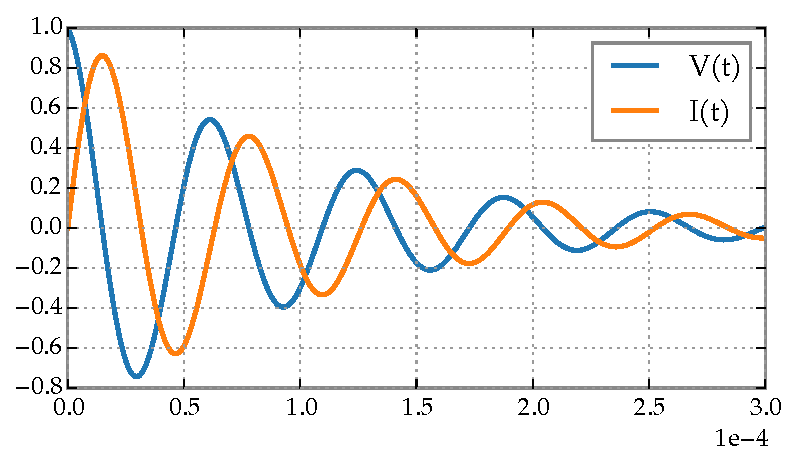
\includegraphics[width=\linewidth]{LC}
\caption{Simulación 1}
\label{fig:sim1}
\end{subfigure}
\begin{subfigure}[b]{0.45\linewidth}
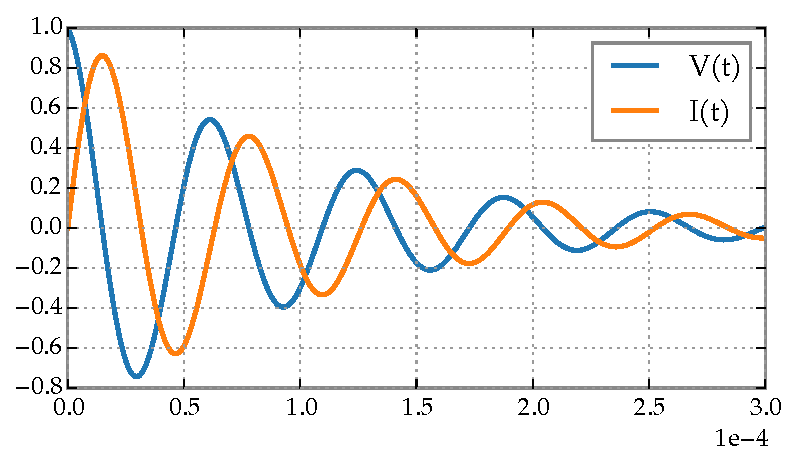
\includegraphics[width=\linewidth]{LC}
\caption{Simulación 2}
\label{fig:sim2}
\end{subfigure}

\begin{subfigure}[b]{0.7\linewidth}
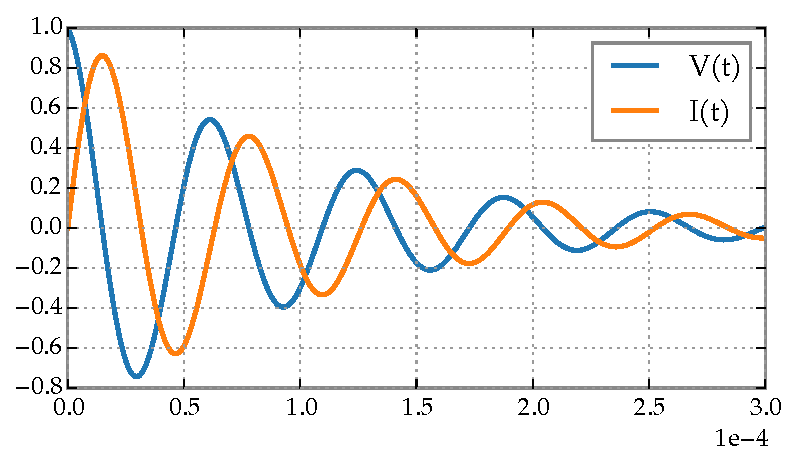
\includegraphics[width=\linewidth]{LC}
\caption{Simulación 3}
\label{fig:sim3}
\end{subfigure}

\caption{Ejemplo de subfiguras. Simulación 1~\subref{fig:sim1}, Simulación 2~\subref{fig:sim2} y Simulación 3~\subref{fig:sim3}.}
\label{fig:simulaciones}
\end{figure}

\section{Tablas}

\begin{table}[h!tb]
\centering
\caption{Ejemplo de tabla.}
\label{tab:ejemplo}
\begin{tabular}{ccccc}
\toprule
\multicolumn{2}{c}{Columna 1 y 2} & Columna 3 & Columna 4 & Columna 5 \\
\midrule
	Dato 1 & Dato 2 & Dato 3 & Dato 4 & Dato 5 \\
\cmidrule(r){1-2} \cmidrule(l){3-5}
	Dato 1 & Dato 2 & Dato 3 & Dato 4 & Dato 5 \\
\bottomrule
\end{tabular}
\end{table}


\section{Ecuaciones}
Ecuación alineada sin numerar
\begin{align*}
a &= b + c + d \\
e &= f + g + h + i
\end{align*}

Ecuación alineada numerada~\eqref{eq:num1},~\eqref{eq:num2}.
\begin{align}
a &= b + c + d \label{eq:num1} \\
e &= f + g + h + i \label{eq:num2}
\end{align}

Múltiples ecuaciones alineadas y con un solo número~\eqref{eq:num3}.
\begin{equation}
\begin{split}
\underbrace{a+\overbrace{b+\cdots}^{=t}+z}
_{\mathrm{total}} &= 
a+{\overbrace{b+\cdots}}^{126}+z \\
%% ecuacion 2
\underbrace{a+\overbrace{b+\cdots}^{=t}+z}
_{\mathrm{total}} &= 
a++b+{\overbrace{c+\cdots}}^{126}+z \\
\end{split}
\label{eq:num3}
\end{equation}

Matrices
\begin{align*}
\dot{\vect{x}} &= \vect{A}\vect{x} + \vect{B}\vect{u} \\
\dot{\vect{y}} &= \vect{C}\vect{x} + \vect{D}\vect{u}
\end{align*}

\begin{align*}
\vect{A} &= \begin{bmatrix}
1 & 0 & 0 \\
0 & 2 & 0 \\
0 & 0 & 3
\end{bmatrix}
%
&
%
\vect{B} &= \begin{bmatrix}
1  \\
0  \\
0 
\end{bmatrix}
%
&
%
\vect{C} &= \begin{bmatrix}
1 & 0 & 0 \\
0 & 2 & 0 \\
0 & 0 & 3
\end{bmatrix}
%
&
%
\vect{D} &= \begin{bmatrix}
1  \\
0  \\
0 
\end{bmatrix}
\end{align*}

\section{Listados de código}

\begin{lstlisting}[style=mlab, caption={código MATLAB.}]
function x = test(a, b)
  x = a + b;
end
\end{lstlisting}

\lstinputlisting[style=mlab, language=Python, caption={Código Python desde archivo.}, lastline=20]{figuras/tanque_LC.py}

% !TEX TS-program = pdflatex
% !TEX encoding = UTF-8 Unicode
% !TEX spellcheck = es_CL
% !TEX root = ../Plantilla_PELN.tex
% Creado por Fabian Inostroza, 2015

\chapter{Estado de avance del trabajo}
\section{Introducción}

\section{Software}

\section{Hardware}
% !TEX TS-program = pdflatex
% !TEX encoding = UTF-8 Unicode
% !TEX spellcheck = es_CL
% !TEX root = ../Plantilla_PELN.tex
% Creado por Fabian Inostroza, 2015

\chapter{Resultados preliminares}

% !TEX TS-program = pdflatex
% !TEX encoding = UTF-8 Unicode
% !TEX spellcheck = es_CL
% !TEX root = ../Plantilla_PELN.tex
% Creado por Fabian Inostroza, 2015
 
\chapter{Carta Gantt}
\section{Carta Gantt propuesta}

\section{Estado de avance}

\section{Ajuste Carta Gantt}

%% !TeX root= ../Plantilla_PELN.tex
% !TEX TS-program = pdflatex
% !TEX encoding = UTF-8 Unicode
% !TEX spellcheck = es_CL
 
\section{Conclusión}

% !TEX TS-program = pdflatex
% !TEX encoding = UTF-8 Unicode
% !TEX spellcheck = es_CL
% !TEX root = Plantilla_PELN.tex
% Creado por Fabian Inostroza, 2015
 
%\section{Bibliografía}
\phantomsection
%\addcontentsline{toc}{section}{\refname} %class article
\addcontentsline{toc}{chapter}{\bibname} % class book
%\bibliographystyle{plain}
\bibliographystyle{IEEEtran-es}
\bibliography{biblio}
%\cleardoublepage
\appendix

% !TEX TS-program = pdflatex
% !TEX encoding = UTF-8 Unicode
% !TEX spellcheck = es_CL
% !TEX root = ../Plantilla_PELN.tex
% Creado por Fabian Inostroza, 2015

%\appendix
\chapter{Anexo}


\end{document}
